
\documentclass[aspectratio=169]{beamer}

% activate me to make slides with no animation
%\documentclass[handout]{beamer}


\usepackage[warn]{mathtext}
\usepackage[T2A]{fontenc}
\usepackage[utf8]{inputenc}
\usepackage[english,russian]{babel}

\usepackage{amssymb}
\usepackage{amsmath}
\usepackage{multirow}
\usepackage{graphicx}
\usepackage{verbatim}
\usepackage{comment} 
\usepackage{minted}

\usepackage{listings}
\lstset{language=Java,
                basicstyle=\footnotesize\ttfamily,
                keywordstyle=\footnotesize\color{blue}\ttfamily,
}


%%%%%%%%%%%%%%%%%%%%%%%%%%%%%%%%%  fix-lstlinebgrd.tex 
\makeatletter
\let\old@lstKV@SwitchCases\lstKV@SwitchCases
\def\lstKV@SwitchCases#1#2#3{}
\makeatother
\usepackage{lstlinebgrd}
\makeatletter
\let\lstKV@SwitchCases\old@lstKV@SwitchCases
        
\lst@Key{numbers}{none}{%
    \def\lst@PlaceNumber{\lst@linebgrd}%
    \lstKV@SwitchCases{#1}%
    {none:\\%
     left:\def\lst@PlaceNumber{\llap{\normalfont
                \lst@numberstyle{\thelstnumber}\kern\lst@numbersep}\lst@linebgrd}\\%
     right:\def\lst@PlaceNumber{\rlap{\normalfont
                \kern\linewidth \kern\lst@numbersep
                \lst@numberstyle{\thelstnumber}}\lst@linebgrd}%
    }{\PackageError{Listings}{Numbers #1 unknown}\@ehc}}
\makeatother
%%%%%%%%%%%%%%%%%%%%%%%%%%%%%%%%%


%%%%%%%%%%%%%%%%%%%%%%%%%%%%%%%%%  bListHL
\makeatletter
%%%%%%%%%%%%%%%%%%%%%%%%%%%%%%%%%%%%%%%%%%%%%%%%%%%%%%%%%%%%%%%%%%%%%%%%%%%%%%
%
% \btIfInRange{number}{range list}{TRUE}{FALSE}
%
% Test in int number <number> is element of a (comma separated) list of ranges
% (such as: {1,3-5,7,10-12,14}) and processes <TRUE> or <FALSE> respectively

\newcount\bt@rangea
\newcount\bt@rangeb

\newcommand\btIfInRange[2]{%
    \global\let\bt@inrange\@secondoftwo%
    \edef\bt@rangelist{#2}%
    \foreach \range in \bt@rangelist {%
        \afterassignment\bt@getrangeb%
        \bt@rangea=0\range\relax%
        \pgfmathtruncatemacro\result{ ( #1 >= \bt@rangea) && (#1 <= \bt@rangeb) }%
        \ifnum\result=1\relax%
            \breakforeach%
            \global\let\bt@inrange\@firstoftwo%
        \fi%
    }%
    \bt@inrange%
}
\newcommand\bt@getrangeb{%
    \@ifnextchar\relax%
        {\bt@rangeb=\bt@rangea}%
        {\@getrangeb}%
}
\def\@getrangeb-#1\relax{%
    \ifx\relax#1\relax%
        \bt@rangeb=100000%   \maxdimen is too large for pgfmath
    \else%
        \bt@rangeb=#1\relax%
    \fi%
}
%%%%%%%%%%%%%%%%%%%%%%%%%%%%%%%%%%%%%%%%%%%%%%%%%%%%%%%%%%%%%%%%%%%%%%%%%%%%%%
%
% \btLstHL<overlay spec>{range list}
%
% TODO BUG: \btLstHL commands can not yet be accumulated if more than one overlay spec match.
%
\newcommand<>{\btLstHL}[1]{%
\only#2{\btIfInRange{\value{lstnumber}}{#1}{\color{yellow}\def\lst@linebgrdcmd{\color@block}}{\def\lst@linebgrdcmd####1####2####3{}}}%
}%

\newcommand<>{\btLstHLG}[1]{%
\only#2{\btIfInRange{\value{lstnumber}}{#1}{\color{green}\def\lst@linebgrdcmd{\color@block}}{\def\lst@linebgrdcmd####1####2####3{}}}%
}%
\makeatother
%%%%%%%%%%%%%%%%%%%%%%%%%%%%%%%%%



\usetheme{CambridgeUS}

% tikz
\usepackage{pgf}
\usepackage{tikz}
\usepackage{tikz-qtree}
\usetikzlibrary{arrows, automata, fit, shapes, shapes.multipart, trees, positioning}

\usepackage{array}
\usepackage{cancel}
\usepackage{hyperref}
\usepackage[normalem]{ulem}


\newtheorem{homeworkmail}[theorem]{Homework, mail}

\newcommand{\showTOC}{
    \begin{frame}[noframenumbering,plain]
        \frametitle{Lecture plan}
        \tableofcontents[currentsection]
    \end{frame}
}

\newcommand{\showTOCSub}{
    \begin{frame}[noframenumbering,plain]
        \frametitle{Lecture plan}
        \tableofcontents[currentsubsection]
    \end{frame}
}


\newcommand{\questiontime}[1]{
    \begin{frame}[noframenumbering,plain]
        \frametitle{Question time}

        Question: #1

        \begin{center}
            \includegraphics[width=0.4\textwidth]{../../common/pics/coins.png}
        \end{center}

        
    \end{frame}
}



\newcommand{\orgNum}{0}
\newcommand{\orgTopic}{org meeting}
\newcommand{\orgKey}{syllabus, contacts}

\newcommand{\introNum}{1}
\newcommand{\introTopic}{introduction to multithreading}
\newcommand{\introKey}{concurrency, parallelism, agents, threads, scheduler, Amdahl's law, race condition, deadlock, wait-for graph}

\newcommand{\basicNum}{2}
\newcommand{\basicTopic}{basic concepts}
\newcommand{\basicKey}{mutex, acquisition order, reentrancy, fairness, data locking, code locking, signalling, condition variable, lost signal, spurious wakeup}

\newcommand{\syncPrimitivesNum}{3}
\newcommand{\syncPrimitivesTopic}{advanced synchronization primitives}
\newcommand{\syncPrimitivesKey}{monitor, latch, barrier, thundering herd, semaphore, read-write lock, thread pool, executor, producer-consumer, fork-join, load balancing}

\newcommand{\patternsNum}{4}
\newcommand{\patternsTopic}{advanced synchronization concepts}
\newcommand{\patternsKey}{interruption, cancellation, partitioning, privatization, replication, thread-local, ownership}

\newcommand{\extraBasicsNum}{5}
\newcommand{\extraBasicsTopic}{additional topics of practical concurrency}
\newcommand{\extraBasicsKey}{documenting protocols and classes, checking concurrent invariants, stress testing, execution trace analysis, estimating required testing effort, static and dynamic checks, scheduling randomization, model checking}

\newcommand{\foundationsNum}{6}
\newcommand{\foundationsTopic}{theoretical foundations of concurrency}
\newcommand{\foundationsKey}{timeline, events, precedence, 2-thread mutual exclusion, deadlock freedom, starvation freedom, N-thread mutual exclusion, sequential objects and specifications, concurrent objects, linearizability}

\newcommand{\foundationsPlusNum}{7}
\newcommand{\foundationsPlusTopic}{progress guarantees, concurrent operations hierarchy, consensus number}
\newcommand{\foundationsPlusKey}{obstruction-free, lock-free, wait-free, safe register, regular register, atomic register, register snapshot, consensus number}

\newcommand{\atomicsNum}{8}
\newcommand{\atomicsTopic}{introduction to atomics}
\newcommand{\atomicsKey}{read-modify-write, get-and-add, compare-and-swap, spin lock, lock-free stack, ABA problem}

% TODO: taxonomy of queues, 

\newcommand{\cacheCoherencyNum}{9}
\newcommand{\cacheCoherencyTopic}{cache coherency}
\newcommand{\cacheCoherencyKey}{cache memory hierarchy, cache coherency protocol, store-buffer, load-buffer, invalidate-queue, memory barrier, hardware memory model, weak memory model, litmus tests}

\newcommand{\langMMNum}{10}
\newcommand{\langMMTopic}{language memory model}
\newcommand{\langMMKey}{compiler optimizations, compiler barriers, language memory model, strict consistency, threads cannot be implemented as a library, visibility, volatile}

\newcommand{\advancedConcurrencyNum}{11}
\newcommand{\advancedConcurrencyTopic}{advanced concurrency}
\newcommand{\advancedConcurrencyKey}{CLH/MCS queue/lock, backoff policies revisited, notify-as-ready, RAT optimization, single LIFO cell optimization, work distribution, work stealing, taxonomy of parallel problems}

\newcommand{\userSpaceThreadingNum}{12}
\newcommand{\userSpaceThreadingTopic}{user-space threading}
\newcommand{\userSpaceThreadingKey}{berkley socket, blocking and non-blocking IO, callback-hell, async-await, continuation-passing-style, fibers/coroutines/green threads, stackful vs stackless}


\newcommand{\designNum}{13}
\newcommand{\designTopic}{designing concurrent systems}
\newcommand{\designKey}{park/unpark, synchronizer, futex/wait-on-address, plan9 approach, race-finders, ForkJoinPool/CoroutineCarriers/UIthread, observability, structured concurrency}

\newcommand{\frameworksAndDistributedNum}{14}
\newcommand{\frameworksAndDistributedTopic}{multi-agent systems}
\newcommand{\frameworksAndDistributedKey}{auto-parallelization languages and frameworks, semi-automatic synchronization, distributed systems, consensus protocols}


\title[]{Lecture \syncPrimitivesNum: \syncPrimitivesTopic}
\subtitle[]{\syncPrimitivesKey}
\author[]{Alexander Filatov\\ filatovaur@gmail.com}

\date{}

\newcommand{\taskRewritePhilosophers}{3.1}


\begin{document}

\begin{frame}
  \titlepage
  \url{https://github.com/Svazars/parallel-programming/blob/main/slides/pdf/l3.pdf}
\end{frame}

\begin{frame}{In previous episode}

We study communication and coordination of different threads in pre-emptive multitasking OS, execution speed is not under our control.

We know the following tools:
\begin{itemize}
    \item \texttt{Thread.start}, \texttt{Thread.join}, \texttt{ReentrantLock}, \texttt{Lock}, \texttt{Condition}
\end{itemize}

We are focusing on the following properties:
\begin{itemize}
    \item Safety, Liveness, Performance
\end{itemize}

For any new concept we must understand
\begin{itemize}
    \item Granularity of coordination (race conditions, level of parallelism)
    \item Blocking API (deadlocks)
    \item Admission policy (fairness, progress)
    \item Locking policy (visibility issues, data races)
    \item Signal send-receive conditions (lost signal, spurious wakeup)
\end{itemize}

We are focusing on high-level policies rather than particular synchronization mechanisms (until Lecture~\advancedConcurrencyNum).

\end{frame}

\begin{frame}{Lecture plan}
\tableofcontents
\end{frame}

\begin{frame}[t]{Disclaimer}

Concurrent programming is evolving branch of Computer Science.

\pause

There are many designs for key synchronization primitives:

\begin{itemize}
    \item ''Monitor classification'' by Buhr et al\footnote<2->{\tiny\url{https://dl.acm.org/doi/10.1145/214037.214100}}
    \item ''Semaphores in Plan 9'' by Mullender and Cox\footnote<2->{\tiny\url{https://swtch.com/semaphore.pdf}}
    \item ''Futexes are tricky'' by Drepper\footnote<2->{\tiny\url{https://www.semanticscholar.org/paper/Futexes-Are-Tricky-Drepper/86253463161f45ea013a501f89c8de36f1a09192}}
\end{itemize}

\pause
We will stick to the Java programming language (built-in monitors) and \texttt{java.util.concurrent} package.

\pause
It is enough to illustrate design space, trade-offs, common correctness problems.

\pause
It is \textbf{not} enough to start concurrency-oriented low-level development in other languages (e.g. C++ stdlib/boost, Golang with plan9 style sema etc).

\end{frame}

\section{Monitor}
\showTOC


\begin{frame}[fragile]{Java monitor}
\framesubtitle{Design}

Effectively \texttt{ReentrantLock + single Condition}

\begin{itemize}
    \item \texttt{MonitorEnter}
    \item \texttt{MonitorExit}
    \item \texttt{wait}
    \item \texttt{notify}
    \item \texttt{notifyAll}
\end{itemize}

\begin{tikzpicture}[remember picture,overlay]
\node[xshift=3.5cm,yshift=-2.5cm] at (current page.center) {\includegraphics[width=0.27\textwidth]{./pics/MonitorJava.png}};
\end{tikzpicture}

\end{frame}

\begin{frame}[fragile]{Java monitor}
\framesubtitle{For every object}

\textbf{Every} Java object have associated built-in monitor.

\begin{minted}{java}
  Object x = new Object();
  synchronized(x) {
    x.wait();
    x.notifyAll();
  }
\end{minted}

Special keyword: \texttt{synchronized} (no \texttt{.lock/unlock}, no try-finally, always structured)

Note: \texttt{Condition} and \texttt{ReentrantLock} are Java objects and they have built-in monitor.

Library-level synchronization and language-level synchronization are \textbf{independent}, do not mix \texttt{notify/signal} and \texttt{wait/await}.

\end{frame}


\begin{frame}[t,fragile]{Java monitor}
\framesubtitle{For every method}

\textbf{Every} Java method could be marked as \texttt{synchronized}.
\begin{minted}{java}
  public void foo() { doStuff(); }
  public synchronized void bar() { doStuffUnderMutex(); }
\end{minted}

It synchronizes on \texttt{this} (instance methods) or \texttt{Class<?>} (static methods):
\begin{minted}{java}
  public synchronized void fooSignature() { doStuff(); }
  public void fooInternal() {
    synchronized(this) {
        doStuff();
    }
  }
\end{minted}

\end{frame}

\questiontime{Is it good or bad to mark methods as thread-safe (\texttt{synchronized} on publicly available signature level?)}

\begin{frame}[t,fragile,noframenumbering]{Java monitor}
\framesubtitle{For every method}

\textbf{Every} Java method could be marked as \texttt{synchronized}.
\begin{minted}{java}
  public void foo() { doStuff(); }
  public synchronized void bar() { doStuffunderMutex(); }
\end{minted}

It synchronizes on \texttt{this} (instance methods) or \texttt{Class<?>} (static methods):
\begin{minted}{java}
  public synchronized void fooSignature() { doStuff(); }
  public void fooInternal() {
    synchronized(this) {
        doStuff();
    }
  }
\end{minted}

Remember that inheritance or \texttt{synchronized(myAwesomeClassInstance)} may break your locking policy and cause a deadlock.

It is common pattern to use \texttt{private final Object lock} and do not expose it as public API.
\end{frame}


\begin{frame}[fragile]{Java monitor}
\framesubtitle{Single-producer single-consumer bounded queue}

\begin{minted}{java}
static Dequeue<Object> buffer = ...
void producer(Object e) {
    synchronized(buffer) {
        while (buffer.size() > N) { buffer.wait(); }
        buffer.offer(e); buffer.notify();
    }
}
Object consumer() {
    synchronized(buffer) {
        while (buffer.isEmpty()) { buffer.wait(); }
        buffer.notify();
        return buffer.poll(); 
    }
}
\end{minted}

\end{frame}

\begin{frame}[t]{Java monitor}
\framesubtitle{Common pitfalls}

\end{frame}

\questiontime{Name 3 key properties that you should understand for any concurrent object}


\begin{frame}[t,noframenumbering]{Java monitor}
\framesubtitle{Common pitfalls}

Correctness(safety):
\begin{itemize}
    \item Blocking \texttt{MonitorEnter}, \texttt{wait} -- deadlock, locking order
    \item Reentrant
    \item Visibility/consistency -- \texttt{synchronized} looks like ''atomic transaction''
    \item Lost signal
    \item Predicate invalidation
    \item Spurious wakeup
\end{itemize}

Progress(liveness):
\begin{itemize}
    \item Admission policy for \texttt{MonitorEnter}/\texttt{MonitorExit} is not specified
    \item Admission policy for \texttt{wait}/\texttt{notify} is not specified
\end{itemize}

Performance:
\begin{itemize}
    \item Lock convoy
    \item Thundering herd \pause (what is it?)
\end{itemize}

\end{frame}


\begin{frame}[t]{Java monitor}
\framesubtitle{Specific pitfalls}

Unintended encapsulation breach:
\begin{itemize}
    \item \texttt{synchronized} methods inheritance
    \item \texttt{synchronized} on object outside of library method
\end{itemize}

Solution: \texttt{private} guards
\
\
\

\pause

Unintended mix of \texttt{java.util.concurrent} and built-in synchronization:
\begin{itemize}
    \item \texttt{wait} vs \texttt{await}
    \item \texttt{synchronized} vs \texttt{lock/unlock}
\end{itemize}

Solution: static analysis (FindBugs/InteliJ IDEA)

\end{frame}

\begin{frame}{Java monitor}
\framesubtitle{Rules of thumb}

Mutual exclusion
\begin{itemize}
    \item If you need ''just mutex'' -- consider using encapsulated object + \texttt{synchronized}
    \begin{itemize}
        \item Save your time with try-finally
        \item Other stuff (built-ins have better monitoring and optimizer-friendly) is debatable
    \end{itemize}

    \pause

    \item Use \texttt{Lock} if you need ''advanced'' properties:
    \begin{itemize}
        \item Fairness (remember, scheduling is counter-intuitive)
        \item Non-structured locking (remember, exceptions are hard)
        \item Polling via \texttt{tryLock} (remember, race conditions are tricky)
    \end{itemize}
\end{itemize}

\pause
Signalling\pause. The story is absolutely the same.

Built-in monitors are ''friendlier'' yet less flexible.

\end{frame}

\begin{frame}{Java monitor}
\framesubtitle{Must-know tool}

Monitor is basic universal building block for concurrent primitives and protocols.

\pause

\begin{homeworkmail}{}{
    Implement every concurrent primitive presented in this course using built-in Java monitor(s). This task is \textbf{not} graded, but your questions are welcome!
}
\end{homeworkmail}

\pause

Monitor combines \textbf{mutual exclusion} and \textbf{signalling} allowing you to make infinite amount of 
\begin{itemize}
    \pause
    \item concurrent design mistakes
    \pause
    \item bugs 
    \pause
    \item performance regressions
\end{itemize}

\pause

Make yourself a favour -- learn basics and then progress on advanced stuff.

\end{frame}

\section{Broadcast}
\showTOC

\begin{frame}[t]{Signalling: broadcast}

\texttt{Lock+Condition} and \texttt{Monitor} provide \texttt{notifyAll}.
\end{frame}

\questiontime{Does \texttt{notifyAll} or \texttt{signalAll} actually force all waiting threads to wake-up?}

\begin{frame}[t,noframenumbering]{Signalling: broadcast}

\texttt{Lock+Condition} and \texttt{Monitor} provide \texttt{notifyAll}.

Effectively threads are ''released'' one-by-one, since they are forced to enter critical section.

\pause
What should we do to perform ''massive release''?

\pause
Use specialized tools!
\end{frame}


\subsection{CountDownLatch}
\showTOCSub

\begin{frame}[fragile]{CountDownLatch}

\begin{center}
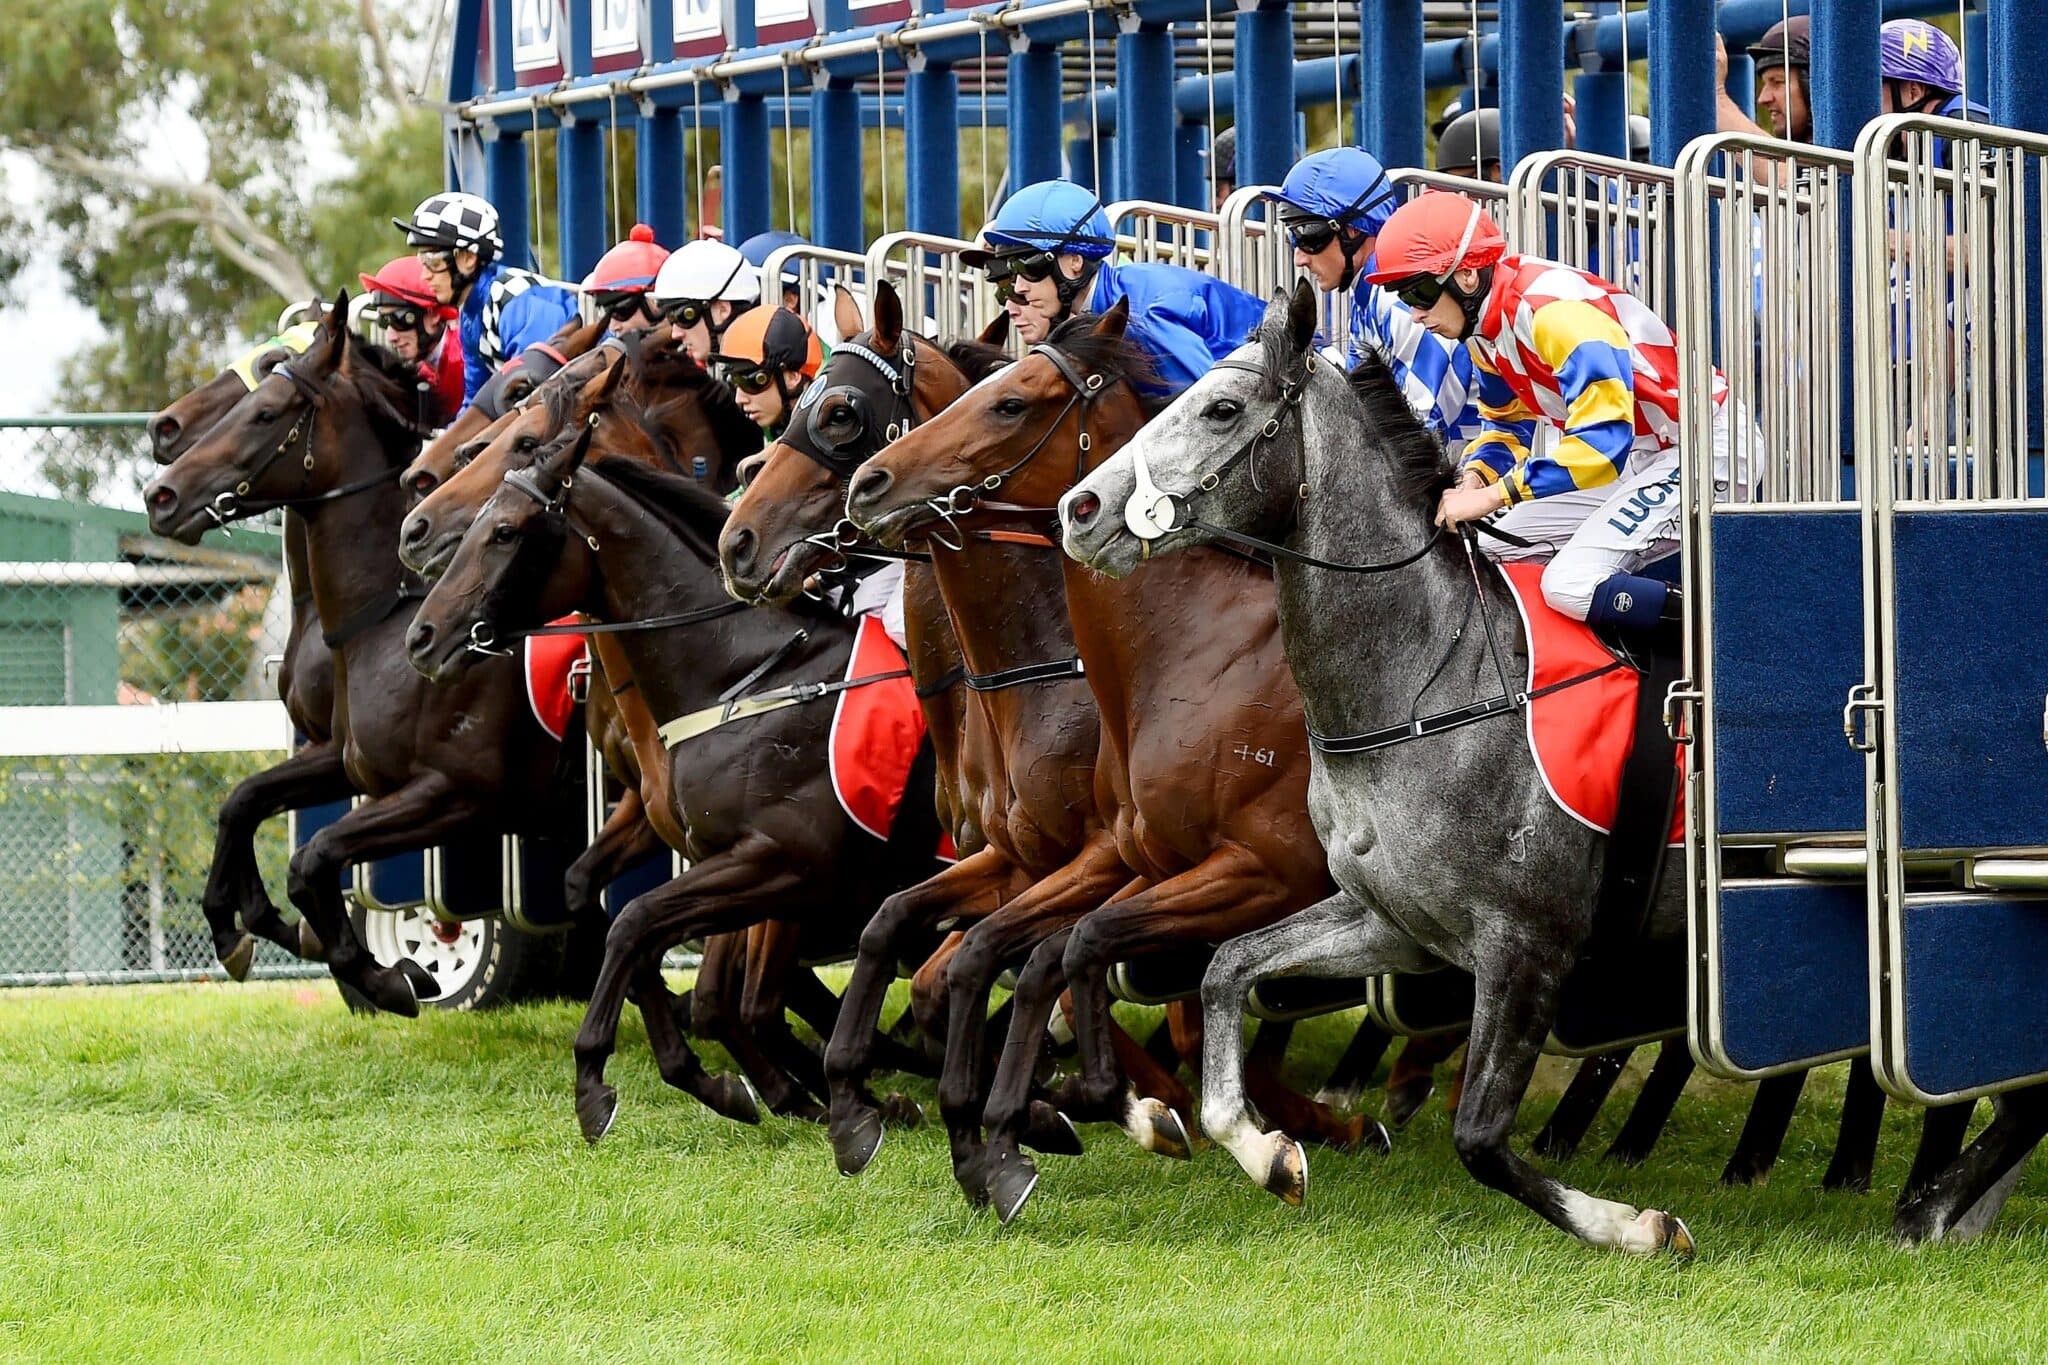
\includegraphics[width=0.8\textwidth]{./pics/horse_race.png}
\end{center}

\end{frame}


\begin{frame}[fragile]{CountDownLatch}

CountDownLatch\footnote{\tiny\url{https://docs.oracle.com/en/java/javase/11/docs/api/java.base/java/util/concurrent/CountDownLatch.html}}

\begin{minted}{java}
  CountDownLatch(int count)
  void await()     // awaits counter == 0
  void countDown() // counter = max(counter - 1, 0)
  long getCount()  // return counter
\end{minted}

Common usage patterns:
\begin{itemize}
    \item \texttt{CountDownLatch(1)} acts as a ''gate'':
    \begin{itemize}
      \item \textbf{closed} (\texttt{counter == 1}) 
      \item \textbf{open} (\texttt{counter == 0})
     \end{itemize}

    \item \texttt{CountDownLatch(N)} acts as a ''all threads ready'' point:
    \begin{itemize}
      \item \textbf{not-yet-ready} (\texttt{counter > 0})
      \item \textbf{ready} (\texttt{counter == 0})
     \end{itemize}
\end{itemize}

%HW: implement via single monitor
%HW: a queue with personal monitors for broadcast
\end{frame}


\begin{frame}[fragile]{CountDownLatch}
\framesubtitle{Example}

\begin{minted}{java}
static CountDownLatch ready = new CountDownLatch(N + 1);
static CountDownLatch start = new CountDownLatch(1);
main() {
    for (i = 0; i < N; i++) new Thread(new Worker(i)).start();
    ready.countDown(); ready.await();
    start.countDown();
}
worker() {
    prepare();
    ready.countDown();
    start.await();
}
\end{minted}
\end{frame}


\subsection{CyclicBarrier}
\showTOCSub

\begin{frame}[t,fragile]{CyclicBarrier}

\texttt{CountDownLatch} is single-use because counter monotonically decreases. 

Some tasks require \texttt{N} iterations of some parallel activity before completion.
\end{frame}

\questiontime{Provide examples of parallelizable tasks that consist of \texttt{N} repeating steps.}


\begin{frame}[t,fragile,noframenumbering]{CyclicBarrier}

\texttt{CountDownLatch} is single-use because counter monotonically decreases. 

Some tasks require \texttt{N} iterations of some parallel activity before completion.

Creating \texttt{ArrayList<CountDownLatch>} is cumbersome.

\end{frame}


\begin{frame}[fragile]{CyclicBarrier}

CyclicBarrier\footnote{\tiny\url{https://docs.oracle.com/en/java/javase/11/docs/api/java.base/java/util/concurrent/CyclicBarrier.html}}

\begin{minted}{java}
  CyclicBarrier(int parties, Runnable barrierAction)
  int await()     
  int getNumberWaiting()  
  int getParties()    
\end{minted}

Common usage patterns: mostly-parallel tasks with sequential coordination
\begin{itemize}
    \item Multiply matrices row-by-row (parallel), handle result (sequential)
    \item Do numerical simulation for \texttt{dt} (parallel), save intermediate result (sequential)
    \item Handle batch of requests (parallel), decide next batch size (sequential)
\end{itemize}

% HW: implement via single monitor
\end{frame}

\begin{frame}[fragile]{CyclicBarrier}
\framesubtitle{Example}

They have example with matrix multiplication right in the javadoc\footnote{{\tiny\url{https://docs.oracle.com/en/java/javase/11/docs/api/java.base/java/util/concurrent/CyclicBarrier.html}}}!
\end{frame}


\subsection{Thundering herd problem}
\showTOCSub


\begin{frame}[fragile]{Thundering herd problem}

\begin{minted}{java}
static Deque<Object> data = ...
static Lock lock = ...
static CountDownLatch dataReady = new CountDownLatch(1);
main(workItems) {
    lock.lock(); 
    try { data.addAll(workItems); } finally { lock.unlock(); }
    dataReady.countDown();
}
worker_i() {
    dataReady.await();
    lock.lock(); 
    try { Object element = data.poll(); } finally { lock.unlock(); }
    process(element);
}
\end{minted}
\end{frame}


\begin{frame}[fragile,noframenumbering]{Thundering herd problem}

\begin{minted}{java}
static Deque<Object> data = ...
static CountDownLatch dataReady = new CountDownLatch(1);
main(workItems) {
    synchronized(data) { 
        data.addAll(workItems); 
    }
    dataReady.countDown();
}
worker_i() {
    dataReady.await();
    synchronized(data) { 
        Object element = data.poll(); 
    }
    process(element);
}
\end{minted}
\end{frame}


\begin{frame}[fragile,noframenumbering]{Thundering herd problem}

    Scenario:
    \begin{itemize}
        \item many threads wake-up because of broadcast 
        \item only few (e.g. single one) make progress
    \end{itemize}

    \pause
    Problem: inefficient utilization of scheduling quantums.

    \pause
    Really similar to lock convoy.

    \pause

    Solution:
    \begin{itemize}
        \item Use broadcasting with care
        \item \texttt{monitor.notifyAll} and \texttt{condition.signalAll} avoid this by moving signalled thread from one queue to another, waking up single ''victim'' on \texttt{MonitorExit/unlock}\footnote<4->{This is called wait morphing}.
    \end{itemize}

    \pause
    Warm reminder: built-in primitives are good and friendly\footnote<5->{High-level overview: ''Compact Java Monitors'' by Dice, Kogan {\url{https://arxiv.org/pdf/2102.04188}}}

\end{frame}

\questiontime{I am confused, could I observe thundering herd problem when using monitors or could not I?}

\section{Group-level concurrency}
\showTOC

\begin{frame}{Group level concurrency}

Mutex divides threads into ''owner'' and ''others''.

Condition divides threads into ''signalled'' and ''others''.

\texttt{CountDownLatch}/\texttt{CyclicBarrier} help to coordinate start/stop for group of threads.

Could we do more?

\begin{itemize}
    \pause
    \item No more than N threads in critical section \pause (semaphore)
    \pause
    \item One exclusive writer and N independent readers \pause (read-write lock)
\end{itemize}

\end{frame}


\subsection{Semaphore}
\showTOCSub

\begin{frame}[fragile]{Semaphore}

\url{https://en.wikipedia.org/wiki/Railway_semaphore_signal}

\begin{center}
\includegraphics[width=0.4\textwidth]{./pics/sema.png}
\end{center}

\end{frame}


\begin{frame}[fragile]{Semaphore}

Semaphore\footnote{\tiny\url{https://docs.oracle.com/en/java/javase/11/docs/api/java.base/java/util/concurrent/Semaphore.html}}

\begin{minted}{java}
  Semaphore(int permits)
  void acquire() // acquire permit, blocks until available
  void release() // release permit
\end{minted}

Important notes:
\begin{itemize}
    \item Perfect to 
    \begin{itemize}
        \item limit number of active threads (parallelism control) 
        \item bound shared resource usage (concurrent access control)
    \end{itemize}    
    \item No ownership -- any thread could \texttt{release} permits
    \item \textit{Binary semaphore} (\texttt{permits == 1}) is very similar to \texttt{NonReentrantLock}
\end{itemize}

\end{frame}

\begin{frame}[fragile]{Semaphore}
\framesubtitle{Example}

\begin{minted}{java}
static Semaphore sema = new Semaphore(N);
static Set<Object> items = ...;
useItem() {
    sema.acquire();
    try {
        synchronized(items) {
            Object item = selectRandom(items);
            items.remove(item);
        }
        use(item);
        synchronized(items) { items.add(item); }
    } finally { sema.release(); }
}
\end{minted}
\end{frame}

\subsection{ReadWriteLock}
\showTOCSub

\begin{frame}[t,fragile]{ReadWriteLock}

ReadWriteLock\footnote{\tiny\url{https://docs.oracle.com/en/java/javase/11/docs/api/java.base/java/util/concurrent/locks/ReadWriteLock.html}}

\begin{minted}{java}
  Lock readLock();
  Lock writeLock();
\end{minted}

Read-mostly data structures:
\begin{itemize}
    \item Concurrent readers, Exclusive writer
\end{itemize}

Design decisions:
\end{frame}

\questiontime{What are the main design decisions for any mutual exclusion primitive?}

\begin{frame}[t,fragile,noframenumbering]{ReadWriteLock}

ReadWriteLock\footnote{\tiny\url{https://docs.oracle.com/en/java/javase/11/docs/api/java.base/java/util/concurrent/locks/ReadWriteLock.html}}

\begin{minted}{java}
  Lock readLock()
  Lock writeLock()
\end{minted}

Read-mostly data structures:
\begin{itemize}
    \item Concurrent readers, Exclusive writer
\end{itemize}

Design decisions:
\begin{itemize}
    \item Reader preference vs. Writer preference
%    TODO-q1: if N active readers why to stop N+1-th reader
%    TODO-q2: if there are X waiting writers and Y waiting readers who should be preferred

    \item Lock upgrade (promotion): readLock -> writeLock

    \item Lock downgrade: writeLock -> readLock

    \item Reentrancy for writers, reentrancy for readers
\end{itemize}

Advanced concurrency control: split threads into two types.
\end{frame}


\begin{frame}[fragile]{ReadWriteLock}
\framesubtitle{Example}

\begin{minted}{java}
static Map<K, V> kv = ...
static ReadWriteLock rw = ..
V get(K k) {
    rw.readLock().lock();
    try {
        return kv.get(k);
    } finally { rw.readLock().unlock(); }
}
void put(K k, V v) {
    rw.writeLock().lock();
    try {
        kv.put(k, v);
    } finally { rw.writeLock().unlock(); }
}
\end{minted}
\end{frame}


\section{Thread pools}
\showTOC

\begin{frame}{Motivation}

\begin{itemize}
    \item \texttt{Thread} is valuable and scarce OS resource. 
    \begin{itemize} \item Caching could help. \end{itemize}
    \item Too many \texttt{Thread}s may slow-down each other (oversubscription). 
    \begin{itemize} \item Soft and hard limits could help. \end{itemize}
    \item Most of the computations do not care which thread is used. 
    \begin{itemize} \item Decoupling tasks from carriers could help. \end{itemize}
    \item \texttt{Thread}s may have purpose and context (name, priority, task-specific limits).
    \begin{itemize} \item  Should be properly reflected in observability API. \end{itemize}
\end{itemize}

\end{frame}


\begin{frame}[fragile]{ThreadFactory}

ThreadFactory\footnote{\tiny\url{https://docs.oracle.com/en/java/javase/11/docs/api/java.base/java/util/concurrent/ThreadFactory.html}}

\begin{minted}{java}
  Thread newThread(Runnable r)
\end{minted}

Key concept: abstracting \texttt{Thread} creation, deletion and maintenance.

Smart words: decoupling \texttt{Thread} life cycle management from business logic.

\end{frame}

\questiontime{\texttt{ThreadFactory} that returns ''previously used'' \texttt{Thread} instance: what are pros and cons?}

\begin{frame}[fragile]{Executor}

Executor\footnote{\tiny\url{https://docs.oracle.com/en/java/javase/11/docs/api/java.base/java/util/concurrent/Executor.html}}

\begin{minted}{java}
  void execute(Runnable command)
\end{minted}

Key concept: abstracting task execution.

Smart words: decoupling business logic (\textbf{what} to do) from implementation (\textbf{how} and \textbf{where} to do) to simplify resource management (\textbf{who} will do).

\end{frame}

\questiontime{\texttt{Executor} does not return \texttt{Future}. Describe valid \texttt{Executor} implementation that indeed does not require \texttt{Future}s. }


\begin{frame}[fragile]{ExecutorService}

ExecutorService\footnote{\tiny\url{https://docs.oracle.com/en/java/javase/11/docs/api/java.base/java/util/concurrent/ExecutorService.html}}

\begin{minted}{java}
  void execute(Runnable command) // implements Executor
  <T> Future<T> submit(Callable<T> task)   
  <T> T invokeAny(Collection<Callable<T>> tasks) // returns any successful
  void shutdown() // no new tasks
  List<Runnable> shutdownNow() // try stop all executing, return all pending
  boolean awaitTermination(long timeout, TimeUnit unit)
\end{minted}

Structured concurrency:
\begin{itemize}
    \item Asynchronous result (\texttt{Future})
    \item Conditional execution (\texttt{invokeAny})
    \item Life cycle management (\texttt{submit}, \texttt{shutdown}, \texttt{awaitTermination})
\end{itemize}

\end{frame}

\questiontime{What if somebody \texttt{submit} task with unhandled exception to \texttt{ExecutorService}? What about other ways to ''destroy'' thread?}

\begin{frame}[fragile]{ScheduledExecutorService}

ScheduledExecutorService\footnote{\tiny\url{https://docs.oracle.com/en/java/javase/11/docs/api/java.base/java/util/concurrent/ScheduledExecutorService.html}}

\begin{minted}{java}
// Value-returning one-shot task that becomes enabled after the given delay
<V> ScheduledFuture<V> schedule(Callable<V> callable, long delay, 
                                TimeUnit unit);
// Periodic action that becomes enabled first after the given initial delay 
// Executions will start after `initialDelay`, then `initialDelay + period` ...
ScheduledFuture<?>  scheduleAtFixedRate(Runnable command, long initialDelay, 
                                        long period, TimeUnit unit);
\end{minted}

Delay and periodic schedule control.

Hint: could be useful for testing, stress measurements and simulating ''workload bursts''.
\end{frame}


\begin{frame}[fragile]{ThreadPools API: summary}

\begin{itemize}
    \item \texttt{ThreadFactory} -- create threads
    \item \texttt{Executor} -- execute tasks
    \item \texttt{ExecutorService}/\texttt{ScheduledExecutorService} -- control task execution (order and resources)
\end{itemize}

\pause

\textbf{Bad news}: you do not know which thread will execute your code.
\begin{itemize}
    \item blocking methods, unexpected lock order, deadlocks, race conditions, data races
\end{itemize}

\pause

\textbf{Good news}: you do not know which thread will execute your code.
\begin{itemize}
    \item under-the-hood synchronization ''just works'', nothing to implement
\end{itemize}

\end{frame}


\begin{frame}[fragile]{ThreadPools API: implementations}

Executors\footnote{\tiny\url{https://docs.oracle.com/en/java/javase/11/docs/api/java.base/java/util/concurrent/Executors.html}}

\begin{minted}{java}
static ExecutorService newFixedThreadPool(int nThreads, ThreadFactory tFactory);
static ExecutorService newSingleThreadExecutor(ThreadFactory threadFactory);
static ExecutorService newCachedThreadPool(ThreadFactory threadFactory);
\end{minted}

\pause

Remember:
\begin{itemize}
    \item Fixed-size thread pools may cause resource deadlock
    \item Single-thread executor not necessarily use the same thread
    \item Caching can cause memory leaks or unintentionally reuse resources (e.g. native-lib-specific resources)
\end{itemize}

Full overview and arbitrary customization available\footnote{\tiny\url{https://docs.oracle.com/en/java/javase/11/docs/api/java.base/java/util/concurrent/ThreadPoolExecutor.html}}

\end{frame}


\begin{frame}[fragile]{ThreadPools API: now you know it}

From now on, you \textbf{must} avoid using \texttt{new Thread()} in your solutions.

\begin{itemize}
    \item Use existing \texttt{ExecutorService}s
    \item Create custom \texttt{ThreadPoolExecutor}s
    \item Encapsulate thread configuration in \texttt{ThreadFactory}
\end{itemize}

\pause

\begin{homeworkcode}{Task~\taskRewritePhilosophers}
Rewrite \texttt{DiningTable.java}\footnote{\tiny\url{https://github.com/Svazars/parallel-programming/blob/main/hw/block1/lec2/dining-philosophers/dining-philosophers/src/main/java/org/nsu/syspro/parprog/base/DiningTable.java}} using \texttt{Executor}s to simplify life cycle management (\texttt{boolean started}, \texttt{boolean shouldStop}).
\end{homeworkcode}

This task is \textbf{independent} from dining philosophers problem, you should refactor existing concurrent code, not invent new one.

\end{frame}


\section{Workload generation}
\showTOC

\begin{frame}{Producer-consumer}

\begin{itemize}
    \item N threads generate work items
    \item M threads process work items
\end{itemize}

\begin{center}
\includegraphics[width=0.7\textwidth]{./pics/prod-cons.png}
\end{center}

BlockingQueue\footnote{\tiny\url{https://docs.oracle.com/en/java/javase/11/docs/api/java.base/java/util/concurrent/BlockingQueue.html}}

\end{frame}

\questiontime{How to ensure that producers and consumers are ''balanced''?}


\begin{frame}{Producer-consumer}

\begin{itemize}
    \item X worker threads
\end{itemize}

Depending on heuristic, every thread either
\begin{itemize}
    \item generate work item
    \item process existing work item
\end{itemize}

\pause

Common problems:
\begin{itemize}
    \item Fixed-size buffer deadlock: 
    \begin{itemize} 
        \item buffer capacity is X
        \item every thread produces no more than 2 elements per iteration
    \end{itemize}

    \item Empty-buffer deadlock: 
    \begin{itemize} 
        \item buffer is empty
        \item every thread heuristically decided to be consumer
    \end{itemize}
\end{itemize}

\end{frame}

\questiontime{How to ensure that producers and consumers reach ''consistent progress''?}

\begin{frame}[t,fragile]{Fork-join}

Fork-join model\footnote{\url{https://en.wikipedia.org/wiki/Fork-join_model}}

\begin{center}
\includegraphics[width=0.65\textwidth]{./pics/fork-join.png}
\end{center}

\end{frame}

\questiontime{How to decide when to stop \texttt{fork}?}


\begin{frame}{Reactive Streams}

\url{https://openjdk.org/jeps/266}

\begin{quote}
The main goal of Reactive Streams is to govern the exchange of stream data across an asynchronous boundary—think passing elements on to another thread or thread-pool
— while ensuring that the receiving side is not forced to buffer arbitrary amounts of data. In other words, back pressure is an integral part of this model in order to 
allow the queues which mediate between threads to be bounded. 
\end{quote}

\texttt{Flow.Publisher<T>}, \texttt{Flow.Subscriber<T>}\footnote{\tiny\url{https://docs.oracle.com/en/java/javase/11/docs/api/java.base/java/util/concurrent/Flow.html}}
\end{frame}


\begin{frame}{Workload generation: takeaways}

\begin{itemize}
    \item Producer-consumer: ''push'' based concurrent system
    \item Fork-join: divide-and-conquer, ''helping hand'' approach
    \item Reactive: ''propagate backpressure'' design 
\end{itemize}

More features -- harder to implement, monitor and control.

\end{frame}


\section{Load balancing}
\showTOC


\begin{frame}{Load balancing}

ThreadPool-based design uses classic timesharing approach: 
\begin{itemize}
    \item there are \texttt{X} tasks (functions) 
    \item \texttt{Y} ''virtual'' executors (threads) which are mapped to
    \item \texttt{Z} ''real'' executors (cores)
\end{itemize}
\pause
There are well-known corner cases:
\begin{itemize}
    \item \texttt{X < Y}: insufficient concurrency (coarse-grained problem)
    \item \texttt{X >> Y}: excessive coordination overheads (too fine-grained approach or too aggressive sub-task creation)
    \item \texttt{Y < Z}: undersubscription (underutilization)
    \item \texttt{Y >> Z}: oversubscription
\end{itemize}
\pause
In any scenario, \texttt{Y} threads have to coordinate task execution:
\begin{itemize}
    \item Eventual progress: every task will be executed
    \item Correctness: every task is executed exactly once
    \item Performance: keep coordination overheads minimal  
\end{itemize}

% TODO: arcticle with perf-oriented designs for over/under scubscription

\end{frame}


\begin{frame}{Load balancing: global queue}
\framesubtitle{Work arbitrage}

Load balancing design:
\begin{itemize}
    \item Single shared thread-safe task queue
    \item Every available \texttt{Worker} gets tasks one-by-one
\end{itemize}

Counter-examples:
\begin{itemize}
    \item Many short tasks
    \item \texttt{Worker}s of varying speeds (energy-efficient and usual cores)
\end{itemize}

\end{frame}

\begin{frame}{Load balancing: global queue + batching}
\framesubtitle{Work arbitrage}

Load balancing design:
\begin{itemize}
    \item Single shared thread-safe task queue
    \item Every available \texttt{Worker} gets tasks in batches (N per request)
\end{itemize}

Counter-examples:
\begin{itemize}
    \item Mix of short and long tasks
    \item \texttt{Worker}s of varying speeds (energy-efficient and usual cores)
\end{itemize}

\end{frame}


\begin{frame}{Load balancing: global queue + batching}
\framesubtitle{Work dealing}

Load balancing design:
\begin{itemize}
    \item Single shared thread-safe task queue
    \item Every available \texttt{Worker} gets tasks in batches (N per request)
    \item Overloaded \texttt{Worker} moves fraction of tasks to global queue
\end{itemize}

Counter-examples:
\begin{itemize}
    \item Few long tasks
    \item Overloaded thread spends CPU for auxiliary coordination
\end{itemize}
\end{frame}

\begin{frame}{Load balancing: work-stealing}

Load balancing design:
\begin{itemize}
    \item Several shared thread-safe task queues (e.g. 1 per \texttt{Worker})
    \item \texttt{Worker} get tasks in batches (N per request) from some queue (''steals'' from neighbour)

\end{itemize}

Not that easy to implement and fine-tune\footnote{\tiny\url{https://shipilev.net/#forkjoin}}. Nontrivial termination protocol.

ForkJoinPool\footnote{\tiny\url{https://docs.oracle.com/en/java/javase/11/docs/api/java.base/java/util/concurrent/ForkJoinPool.html}}

\end{frame}


\section{Summary}

\begin{frame}{Summary}

Mutual exclusion and signalling combined into single universal primitive: monitor

Java language has special support for built-in monitors: \texttt{synchronized} keyword 

Bulk thread notification:
\begin{itemize}
    \item \texttt{CountDownLatch}, \texttt{CyclicBarrier}
    \item Thundering herd problem
\end{itemize}

Tools for fine-grained group-level thread control:
\begin{itemize}
    \item \texttt{Semaphore}, \texttt{ReadWritelock}
\end{itemize}

Universal API for thread/task management:
\begin{itemize}
    \item \texttt{ThreadFactory}, \texttt{Executor}, \texttt{ExecutorService}
\end{itemize}

Different ways to generate workload concurrently:
\begin{itemize}
    \item Producer-consumer, Fork-join, Reactive Streams
\end{itemize}

Designs for efficient concurrent load balancing:
\begin{itemize}
    \item Work arbitrage, Work dealing, Work stealing
\end{itemize}
\end{frame}


\begin{frame}{Summary: homework}

\begin{homeworkmail}{}{
    Implement every concurrent primitive presented in this course using built-in Java monitor(s). This task is \textbf{not} graded, but your questions are welcome!
}
\end{homeworkmail}

\begin{homeworkcode}{Task~\taskRewritePhilosophers}
Rewrite \texttt{DiningTable.java}\footnote{\tiny\url{https://github.com/Svazars/parallel-programming/blob/main/hw/block1/lec2/dining-philosophers/dining-philosophers/src/main/java/org/nsu/syspro/parprog/base/DiningTable.java}} using \texttt{Executor}s to simplify life cycle management (\texttt{boolean started}, \texttt{boolean shouldStop}).
\end{homeworkcode}

\end{frame}


\end{document}
